    \hypertarget{expressions-ruxe9guliuxe8res-et-le-module-re}{%
\section{\texorpdfstring{Expressions régulières et le module
\texttt{re}}{Expressions régulières et le module re}}\label{expressions-ruxe9guliuxe8res-et-le-module-re}}

    \hypertarget{compluxe9ment---niveau-basique}{%
\subsection{Complément - niveau
basique}\label{compluxe9ment---niveau-basique}}

    \hypertarget{avertissement}{%
\subsubsection{Avertissement}\label{avertissement}}

Après avoir joué ce cours plusieurs années de suite, l'expérience nous
montre qu'il est difficile de trouver le bon moment pour appréhender les
expressions régulières.\\

D'un côté il s'agit de manipulations de chaînes de caractères, mais d'un
autre cela nécessite de créer des instances de classes, et donc d'avoir
vu la programmation orientée objet. Du coup, les premières années nous
les avions étudiées tout à la fin du cours, ce qui avait pu créer une
certaine frustration.\\

C'est pourquoi nous avons décidé à présent de les étudier très tôt, dans
cette séquence consacrée aux chaines de caractères. Les étudiants qui
seraient décontenancés par ce contenu sont invités à y retourner après
la semaine 6, consacrée à la programmation objet.\\

Il nous semble important de savoir que ces fonctionnalités existent dans
le langage, le détail de leur utilisation n'est toutefois pas critique,
et on peut parfaitement faire l'impasse sur ce complément en première
lecture.\\

    Une expression régulière est un objet mathématique permettant de décrire
un ensemble de textes qui possèdent des propriétés communes. Par
exemple, s'il vous arrive d'utiliser un terminal, et que vous tapez

\begin{verbatim}
$ dir *.txt
\end{verbatim}

(ou \texttt{ls\ *.txt} sur linux ou mac), vous utilisez l'expression
régulière \texttt{*.txt} qui désigne tous les fichiers dont le nom se
termine par \texttt{.txt}. On dit que l'expression régulière
\emph{filtre} toutes les chaînes qui se terminent par \texttt{.txt}
(l'expression anglaise consacrée est le \emph{pattern matching}).\\

    Le langage Perl a été le premier à populariser l'utilisation des
expressions régulières en les supportant nativement dans le langage, et
non au travers d'une librairie. En python, les expressions régulières
sont disponibles de manière plus traditionnelle, via le module
\texttt{re} (regular expressions) de la librairie standard. Le propos de
ce complément est de vous en donner une première introduction.

    \begin{Verbatim}[commandchars=\\\{\}]
{\color{incolor}In [{\color{incolor}1}]:} \PY{k+kn}{import} \PY{n+nn}{re}
\end{Verbatim}


    \hypertarget{survol}{%
\subsubsection{Survol}\label{survol}}

    Pour ceux qui ne souhaitent pas approfondir, voici un premier exemple;
on cherche à savoir si un objet \texttt{chaine} est ou non de la forme
\texttt{*-*.txt}, et si oui, à calculer la partie de la chaine qui
remplace le \texttt{*}~:

    \begin{Verbatim}[commandchars=\\\{\}]
{\color{incolor}In [{\color{incolor}2}]:} \PY{c+c1}{\PYZsh{} un objet \PYZsq{}expression régulière\PYZsq{} \PYZhy{} on dit aussi \PYZdq{}pattern\PYZdq{}}
        \PY{n}{regexp} \PY{o}{=} \PY{l+s+s2}{\PYZdq{}}\PY{l+s+s2}{(.*)\PYZhy{}(.*)}\PY{l+s+s2}{\PYZbs{}}\PY{l+s+s2}{.txt}\PY{l+s+s2}{\PYZdq{}}
\end{Verbatim}


    \begin{Verbatim}[commandchars=\\\{\}]
{\color{incolor}In [{\color{incolor}3}]:} \PY{c+c1}{\PYZsh{} la chaine de départ}
        \PY{n}{chaine} \PY{o}{=} \PY{l+s+s2}{\PYZdq{}}\PY{l+s+s2}{abcdef.txt}\PY{l+s+s2}{\PYZdq{}}
\end{Verbatim}


    \begin{Verbatim}[commandchars=\\\{\}]
{\color{incolor}In [{\color{incolor}4}]:} \PY{c+c1}{\PYZsh{} la fonction qui calcule si la chaine \PYZdq{}matche\PYZdq{} le pattern}
        \PY{n}{match} \PY{o}{=} \PY{n}{re}\PY{o}{.}\PY{n}{match}\PY{p}{(}\PY{n}{regexp}\PY{p}{,} \PY{n}{chaine}\PY{p}{)}
        \PY{n}{match} \PY{o+ow}{is} \PY{k+kc}{None}
\end{Verbatim}


\begin{Verbatim}[commandchars=\\\{\}]
{\color{outcolor}Out[{\color{outcolor}4}]:} True
\end{Verbatim}
            
    Le fait que l'objet \texttt{match} vaut \texttt{None} indique que la
chaine n'est pas de la bonne forme (il manque un \texttt{-} dans le
nom); avec une autre chaine par contre~:

    \begin{Verbatim}[commandchars=\\\{\}]
{\color{incolor}In [{\color{incolor}5}]:} \PY{c+c1}{\PYZsh{} la chaine de départ}
        \PY{n}{chaine} \PY{o}{=} \PY{l+s+s2}{\PYZdq{}}\PY{l+s+s2}{abc\PYZhy{}def.txt}\PY{l+s+s2}{\PYZdq{}}
\end{Verbatim}


    \begin{Verbatim}[commandchars=\\\{\}]
{\color{incolor}In [{\color{incolor}6}]:} \PY{n}{match} \PY{o}{=} \PY{n}{re}\PY{o}{.}\PY{n}{match}\PY{p}{(}\PY{n}{regexp}\PY{p}{,} \PY{n}{chaine}\PY{p}{)}
        \PY{n}{match} \PY{o+ow}{is} \PY{k+kc}{None}
\end{Verbatim}


\begin{Verbatim}[commandchars=\\\{\}]
{\color{outcolor}Out[{\color{outcolor}6}]:} False
\end{Verbatim}
            
    Ici \texttt{match} est un objet, qui nous permet ensuite d'``extraire''
les différentes parties, comme ceci~:

    \begin{Verbatim}[commandchars=\\\{\}]
{\color{incolor}In [{\color{incolor}7}]:} \PY{n}{match}\PY{p}{[}\PY{l+m+mi}{1}\PY{p}{]}
\end{Verbatim}


\begin{Verbatim}[commandchars=\\\{\}]
{\color{outcolor}Out[{\color{outcolor}7}]:} 'abc'
\end{Verbatim}
            
    \begin{Verbatim}[commandchars=\\\{\}]
{\color{incolor}In [{\color{incolor}8}]:} \PY{n}{match}\PY{p}{[}\PY{l+m+mi}{2}\PY{p}{]}
\end{Verbatim}


\begin{Verbatim}[commandchars=\\\{\}]
{\color{outcolor}Out[{\color{outcolor}8}]:} 'def'
\end{Verbatim}
            
    Bien sûr on peut faire des choses beaucoup plus élaborées avec
\texttt{re}, mais en première lecture cette introduction doit vous
suffire pour avoir une idée de ce qu'on peut faire avec les expressions
régulières.

    \hypertarget{compluxe9ment---niveau-intermuxe9diaire}{%
\subsection{Complément - niveau
intermédiaire}\label{compluxe9ment---niveau-intermuxe9diaire}}

    Approfondissons à présent:\\

    Dans un terminal, \texttt{*.txt} est une expression régulière très
simple. Le module \texttt{re} fournit le moyen de construire des
expressions régulières très élaborées et plus puissantes que ce que
supporte le terminal. C'est pourquoi la syntaxe des regexps de
\texttt{re} est un peu différente. Par exemple comme on vient de le
voir, pour filtrer la même famille de chaînes que \texttt{*-*.txt} avec
le module \texttt{re}, il nous a fallu écrire l'expression régulière
sous une forme légèrement différente.\\

    Je vous conseille d'avoir sous la main la
\href{https://docs.python.org/3/library/re.html}{documentation du module
\texttt{re}} pendant que vous lisez ce complément.

    \hypertarget{avertissement}{%
\subsubsection{Avertissement}\label{avertissement}}

    Dans ce complément nous serons amenés à utiliser des traits qui
dépendent du LOCALE, c'est-à-dire, pour faire simple, de la
configuration de l'ordinateur vis-à-vis de la langue.\\

Tant que vous exécutez ceci dans le notebook sur la plateforme, en
principe tout le monde verra exactement la même chose. Par contre, si
vous faites tourner le même code sur votre ordinateur, il se peut que
vous obteniez des résultats légèrement différents.

    \hypertarget{un-exemple-simple}{%
\subsubsection{Un exemple simple}\label{un-exemple-simple}}

    \hypertarget{findall}{%
\subparagraph{\texorpdfstring{\texttt{findall}}{findall}}\label{findall}}

    On se donne deux exemples de chaînes

    \begin{Verbatim}[commandchars=\\\{\}]
{\color{incolor}In [{\color{incolor}9}]:} \PY{n}{sentences} \PY{o}{=} \PY{p}{[}\PY{l+s+s1}{\PYZsq{}}\PY{l+s+s1}{Lacus a donec, vitae gravida proin sociis.}\PY{l+s+s1}{\PYZsq{}}\PY{p}{,} 
                     \PY{l+s+s1}{\PYZsq{}}\PY{l+s+s1}{Neque ipsum! rhoncus cras quam.}\PY{l+s+s1}{\PYZsq{}}\PY{p}{]}
\end{Verbatim}


    On peut \textbf{chercher tous} les mots se terminant par \texttt{a} ou
\texttt{m} dans une chaîne avec \texttt{findall}

    \begin{Verbatim}[commandchars=\\\{\}]
{\color{incolor}In [{\color{incolor}10}]:} \PY{k}{for} \PY{n}{sentence} \PY{o+ow}{in} \PY{n}{sentences}\PY{p}{:}
             \PY{n+nb}{print}\PY{p}{(}\PY{n}{f}\PY{l+s+s2}{\PYZdq{}}\PY{l+s+s2}{\PYZhy{}\PYZhy{}\PYZhy{}\PYZhy{} dans \PYZgt{}}\PY{l+s+si}{\PYZob{}sentence\PYZcb{}}\PY{l+s+s2}{\PYZlt{}}\PY{l+s+s2}{\PYZdq{}}\PY{p}{)}
             \PY{n+nb}{print}\PY{p}{(}\PY{n}{re}\PY{o}{.}\PY{n}{findall}\PY{p}{(}\PY{l+s+sa}{r}\PY{l+s+s2}{\PYZdq{}}\PY{l+s+s2}{\PYZbs{}}\PY{l+s+s2}{w*[am]}\PY{l+s+s2}{\PYZbs{}}\PY{l+s+s2}{W}\PY{l+s+s2}{\PYZdq{}}\PY{p}{,} \PY{n}{sentence}\PY{p}{)}\PY{p}{)}
\end{Verbatim}


    \begin{Verbatim}[commandchars=\\\{\}]
---- dans >Lacus a donec, vitae gravida proin sociis.<
['a ', 'gravida ']
---- dans >Neque ipsum! rhoncus cras quam.<
['ipsum!', 'quam.']

    \end{Verbatim}

    Ce code permet de chercher toutes (\texttt{findall}) les occurrences de
l'expression régulière, qui ici est définie par le \emph{raw-string}

\begin{verbatim}
r"\w*[am]\W"
\end{verbatim}

Nous verrons tout à l'heure comment fabriquer des expressions régulières
plus en détail, mais pour démystifier au moins celle-ci, on a mis bout à
bout les morceaux suivants.

\begin{itemize}
	\item 
	\texttt{\textbackslash{}w*} : on veut
	trouver une sous-chaîne qui commence par un nombre quelconque, y compris
	nul (\texttt{*}) de caractères alphanumériques
	(\texttt{\textbackslash{}w}). Ceci est défini en fonction de votre
	LOCALE, on y reviendra.
	\item
	\texttt{{[}am{]}} : immédiatement après, il
	nous faut trouver un caratère \texttt{a} ou \texttt{m}.
	\item
	\texttt{\textbackslash{}W} : et enfin, il nous faut un caractère qui ne
	soit \textbf{pas} alphanumérique. Ceci est important puisqu'on cherche
	les mots qui \textbf{se terminent} par un \texttt{a} ou un \texttt{m},
	si on ne le mettait pas on obtiendrait ceci
\end{itemize}

    \begin{Verbatim}[commandchars=\\\{\}]
{\color{incolor}In [{\color{incolor}11}]:} \PY{c+c1}{\PYZsh{} le \PYZbs{}W final est important}
         \PY{c+c1}{\PYZsh{} voici ce qu\PYZsq{}on obtient si on l\PYZsq{}omet}
         \PY{k}{for} \PY{n}{sentence} \PY{o+ow}{in} \PY{n}{sentences}\PY{p}{:}
             \PY{n+nb}{print}\PY{p}{(}\PY{n}{f}\PY{l+s+s2}{\PYZdq{}}\PY{l+s+s2}{\PYZhy{}\PYZhy{}\PYZhy{}\PYZhy{} dans \PYZgt{}}\PY{l+s+si}{\PYZob{}sentence\PYZcb{}}\PY{l+s+s2}{\PYZlt{}}\PY{l+s+s2}{\PYZdq{}}\PY{p}{)}
             \PY{n+nb}{print}\PY{p}{(}\PY{n}{re}\PY{o}{.}\PY{n}{findall}\PY{p}{(}\PY{l+s+sa}{r}\PY{l+s+s2}{\PYZdq{}}\PY{l+s+s2}{\PYZbs{}}\PY{l+s+s2}{w*[am]}\PY{l+s+s2}{\PYZdq{}}\PY{p}{,} \PY{n}{sentence}\PY{p}{)}\PY{p}{)}
\end{Verbatim}


    \begin{Verbatim}[commandchars=\\\{\}]
---- dans >Lacus a donec, vitae gravida proin sociis.<
['La', 'a', 'vita', 'gravida']
---- dans >Neque ipsum! rhoncus cras quam.<
['ipsum', 'cra', 'quam']

    \end{Verbatim}

    \hypertarget{split}{%
\subparagraph{\texorpdfstring{\texttt{split}}{split}\\\\}\label{split}}

    Une autre forme simple d'utilisation des regexps est \texttt{re.split},
qui fournit une fonctionnalité voisine de \texttt{str.split}, mais ou
les séparateurs sont exprimés comme une expression régulière

    \begin{Verbatim}[commandchars=\\\{\}]
{\color{incolor}In [{\color{incolor}12}]:} \PY{k}{for} \PY{n}{sentence} \PY{o+ow}{in} \PY{n}{sentences}\PY{p}{:}
             \PY{n+nb}{print}\PY{p}{(}\PY{n}{f}\PY{l+s+s2}{\PYZdq{}}\PY{l+s+s2}{\PYZhy{}\PYZhy{}\PYZhy{}\PYZhy{} dans \PYZgt{}}\PY{l+s+si}{\PYZob{}sentence\PYZcb{}}\PY{l+s+s2}{\PYZlt{}}\PY{l+s+s2}{\PYZdq{}}\PY{p}{)}
             \PY{n+nb}{print}\PY{p}{(}\PY{n}{re}\PY{o}{.}\PY{n}{split}\PY{p}{(}\PY{l+s+sa}{r}\PY{l+s+s2}{\PYZdq{}}\PY{l+s+s2}{\PYZbs{}}\PY{l+s+s2}{W+}\PY{l+s+s2}{\PYZdq{}}\PY{p}{,} \PY{n}{sentence}\PY{p}{)}\PY{p}{)}
             \PY{n+nb}{print}\PY{p}{(}\PY{p}{)}
\end{Verbatim}


    \begin{Verbatim}[commandchars=\\\{\}]
---- dans >Lacus a donec, vitae gravida proin sociis.<
['Lacus', 'a', 'donec', 'vitae', 'gravida', 'proin', 'sociis', '']

---- dans >Neque ipsum! rhoncus cras quam.<
['Neque', 'ipsum', 'rhoncus', 'cras', 'quam', '']


    \end{Verbatim}

    Ici l'expression régulière, qui bien sûr décrit le séparateur, est
simplement \texttt{\textbackslash{}W+} c'est-à-dire toute suite d'au
moins un caractère non alphanumérique.\\

Nous avons donc là un moyen simple, et plus puissant que
\texttt{str.split}, de couper un texte en mots.

    \hypertarget{sub}{%
\subparagraph{\texorpdfstring{\texttt{sub}}{sub}\\\\}\label{sub}}

    Une troisième méthode utilitaire est \texttt{re.sub} qui permet de
remplacer les occurrences d'une \emph{regexp}, comme par exemple

    \begin{Verbatim}[commandchars=\\\{\}]
{\color{incolor}In [{\color{incolor}13}]:} \PY{k}{for} \PY{n}{sentence} \PY{o+ow}{in} \PY{n}{sentences}\PY{p}{:}
             \PY{n+nb}{print}\PY{p}{(}\PY{n}{f}\PY{l+s+s2}{\PYZdq{}}\PY{l+s+s2}{\PYZhy{}\PYZhy{}\PYZhy{}\PYZhy{} dans \PYZgt{}}\PY{l+s+si}{\PYZob{}sentence\PYZcb{}}\PY{l+s+s2}{\PYZlt{}}\PY{l+s+s2}{\PYZdq{}}\PY{p}{)}
             \PY{n+nb}{print}\PY{p}{(}\PY{n}{re}\PY{o}{.}\PY{n}{sub}\PY{p}{(}\PY{l+s+sa}{r}\PY{l+s+s2}{\PYZdq{}}\PY{l+s+s2}{(}\PY{l+s+s2}{\PYZbs{}}\PY{l+s+s2}{w+)}\PY{l+s+s2}{\PYZdq{}}\PY{p}{,} \PY{l+s+sa}{r}\PY{l+s+s2}{\PYZdq{}}\PY{l+s+s2}{X}\PY{l+s+s2}{\PYZbs{}}\PY{l+s+s2}{1Y}\PY{l+s+s2}{\PYZdq{}}\PY{p}{,} \PY{n}{sentence}\PY{p}{)}\PY{p}{)}
             \PY{n+nb}{print}\PY{p}{(}\PY{p}{)}
\end{Verbatim}


    \begin{Verbatim}[commandchars=\\\{\}]
---- dans >Lacus a donec, vitae gravida proin sociis.<
XLacusY XaY XdonecY, XvitaeY XgravidaY XproinY XsociisY.

---- dans >Neque ipsum! rhoncus cras quam.<
XNequeY XipsumY! XrhoncusY XcrasY XquamY.


    \end{Verbatim}

    Ici, l'expression régulière (le premier argument) contient un
\textbf{groupe}~: on a utilisé des parenthèses autour du
\texttt{\textbackslash{}w+}. Le second argument est la chaîne de
remplacement, dans laquelle on a fait \textbf{référence au groupe} en
écrivant \texttt{\textbackslash{}1}, qui veut dire tout simplement ``le
premier groupe''.\\

Donc au final, l'effet de cet appel est d'entourer toutes les suites de
caractères alphanumériques par \texttt{X} et \texttt{Y}.

    \hypertarget{pourquoi-un-raw-string}{%
\subparagraph{\texorpdfstring{Pourquoi un \emph{raw-string}
?}{Pourquoi un raw-string ?}\\\\}\label{pourquoi-un-raw-string}}

    En guise de digression, il n'y a aucune obligation à utiliser un
\emph{raw-string}, d'ailleurs on rappelle qu'il n'y a pas de différence
de nature entre un \emph{raw-string} et une chaîne usuelle

    \begin{Verbatim}[commandchars=\\\{\}]
{\color{incolor}In [{\color{incolor}14}]:} \PY{n}{raw} \PY{o}{=} \PY{l+s+sa}{r}\PY{l+s+s1}{\PYZsq{}}\PY{l+s+s1}{abc}\PY{l+s+s1}{\PYZsq{}}
         \PY{n}{regular} \PY{o}{=} \PY{l+s+s1}{\PYZsq{}}\PY{l+s+s1}{abc}\PY{l+s+s1}{\PYZsq{}}
         \PY{c+c1}{\PYZsh{} comme on a pris une \PYZsq{}petite\PYZsq{} chaîne ce sont les mêmes objets}
         \PY{n+nb}{print}\PY{p}{(}\PY{n}{f}\PY{l+s+s2}{\PYZdq{}}\PY{l+s+s2}{both compared with is → }\PY{l+s+s2}{\PYZob{}}\PY{l+s+s2}{raw is regular\PYZcb{}}\PY{l+s+s2}{\PYZdq{}}\PY{p}{)}
         \PY{c+c1}{\PYZsh{} et donc a fortiori}
         \PY{n+nb}{print}\PY{p}{(}\PY{n}{f}\PY{l+s+s2}{\PYZdq{}}\PY{l+s+s2}{both compared with == → }\PY{l+s+s2}{\PYZob{}}\PY{l+s+s2}{raw == regular\PYZcb{}}\PY{l+s+s2}{\PYZdq{}}\PY{p}{)}
\end{Verbatim}


    \begin{Verbatim}[commandchars=\\\{\}]
both compared with is → True
both compared with == → True

    \end{Verbatim}

    Il se trouve que le \emph{backslash} \texttt{\textbackslash{}} à
l'intérieur des expressions régulières est d'un usage assez courant - on
l'a vu déjà plusieurs fois. C'est pourquoi on \textbf{utilise
fréquemment un \emph{raw-string}} pour décrire une expression régulière,
et en général à chaque fois qu'elle comporte un \emph{backslash}. On
rappelle que le raw-string désactive l'interprétation des
\texttt{\textbackslash{}} à l'intérieur de la chaîne, par exemple,
\texttt{\textbackslash{}t} est interprété comme un caractère de
tabulation. Sans raw-string, il faut doubler tous les
\texttt{\textbackslash{}} pour qu'il n'y ait pas d'interprétation.

    \hypertarget{un-deuxiuxe8me-exemple}{%
\subsubsection{Un deuxième exemple}\label{un-deuxiuxe8me-exemple}}

    Nous allons maintenant voir comment on peut d'abord vérifier si une
chaîne est conforme au critère défini par l'expression régulière, mais
aussi \emph{extraire} les morceaux de la chaîne qui correspondent aux
différentes parties de l'expression.\\

Pour cela, supposons qu'on s'intéresse aux chaînes qui comportent 5
parties, une suite de chiffres, une suite de lettres, des chiffres à
nouveau, des lettres et enfin de nouveau des chiffres.\\

    Pour cela on considère ces trois chaines en entrée

    \begin{Verbatim}[commandchars=\\\{\}]
{\color{incolor}In [{\color{incolor}15}]:} \PY{n}{samples} \PY{o}{=} \PY{p}{[}\PY{l+s+s1}{\PYZsq{}}\PY{l+s+s1}{890hj000nnm890}\PY{l+s+s1}{\PYZsq{}}\PY{p}{,}    \PY{c+c1}{\PYZsh{} cette entrée convient}
                   \PY{l+s+s1}{\PYZsq{}}\PY{l+s+s1}{123abc456def789}\PY{l+s+s1}{\PYZsq{}}\PY{p}{,}   \PY{c+c1}{\PYZsh{} celle\PYZhy{}ci aussi}
                   \PY{l+s+s1}{\PYZsq{}}\PY{l+s+s1}{8090abababab879}\PY{l+s+s1}{\PYZsq{}}\PY{p}{,}   \PY{c+c1}{\PYZsh{} celle\PYZhy{}ci non}
                   \PY{p}{]}
\end{Verbatim}


    \hypertarget{match}{%
\subparagraph{\texorpdfstring{\texttt{match}}{match}}\label{match}}

    Pour commencer, voyons que l'on peut facilement \textbf{vérifier si une
chaîne vérifie} ou non le critère.

    \begin{Verbatim}[commandchars=\\\{\}]
{\color{incolor}In [{\color{incolor}16}]:} \PY{n}{regexp1} \PY{o}{=} \PY{l+s+s2}{\PYZdq{}}\PY{l+s+s2}{[0\PYZhy{}9]+[A\PYZhy{}Za\PYZhy{}z]+[0\PYZhy{}9]+[A\PYZhy{}Za\PYZhy{}z]+[0\PYZhy{}9]+}\PY{l+s+s2}{\PYZdq{}}
\end{Verbatim}


    Si on applique cette expression régulière à toutes nos entrées

    \begin{Verbatim}[commandchars=\\\{\}]
{\color{incolor}In [{\color{incolor}17}]:} \PY{k}{for} \PY{n}{sample} \PY{o+ow}{in} \PY{n}{samples}\PY{p}{:}
             \PY{n}{match} \PY{o}{=} \PY{n}{re}\PY{o}{.}\PY{n}{match}\PY{p}{(}\PY{n}{regexp1}\PY{p}{,} \PY{n}{sample}\PY{p}{)}
             \PY{n+nb}{print}\PY{p}{(}\PY{n}{f}\PY{l+s+s2}{\PYZdq{}}\PY{l+s+si}{\PYZob{}sample:16s\PYZcb{}}\PY{l+s+s2}{ → }\PY{l+s+si}{\PYZob{}match\PYZcb{}}\PY{l+s+s2}{\PYZdq{}}\PY{p}{)}
\end{Verbatim}


    \begin{Verbatim}[commandchars=\\\{\}]
890hj000nnm890   → <\_sre.SRE\_Match object; span=(0, 14), match='890hj000nnm890'>
123abc456def789  → <\_sre.SRE\_Match object; span=(0, 15), match='123abc456def789'>
8090abababab879  → None

    \end{Verbatim}

    Pour rendre ce résultat un peu plus lisible nous nous définissons une
petite fonction de confort.

    \begin{Verbatim}[commandchars=\\\{\}]
{\color{incolor}In [{\color{incolor}18}]:} \PY{c+c1}{\PYZsh{} pour simplement visualiser si on a un match ou pas}
         \PY{k}{def} \PY{n+nf}{nice}\PY{p}{(}\PY{n}{match}\PY{p}{)}\PY{p}{:}
             \PY{c+c1}{\PYZsh{} le retour de re.match est soit None, soit un objet match}
             \PY{k}{return} \PY{l+s+s2}{\PYZdq{}}\PY{l+s+s2}{no}\PY{l+s+s2}{\PYZdq{}} \PY{k}{if} \PY{n}{match} \PY{o+ow}{is} \PY{k+kc}{None} \PY{k}{else} \PY{l+s+s2}{\PYZdq{}}\PY{l+s+s2}{Match!}\PY{l+s+s2}{\PYZdq{}}
\end{Verbatim}


    Avec quoi on peut refaire l'essai sur toutes nos entrées.

    \begin{Verbatim}[commandchars=\\\{\}]
{\color{incolor}In [{\color{incolor}19}]:} \PY{c+c1}{\PYZsh{} la même chose mais un peu moins encombrant}
         \PY{n+nb}{print}\PY{p}{(}\PY{n}{f}\PY{l+s+s2}{\PYZdq{}}\PY{l+s+s2}{REGEXP=}\PY{l+s+si}{\PYZob{}regexp1\PYZcb{}}\PY{l+s+se}{\PYZbs{}n}\PY{l+s+s2}{\PYZdq{}}\PY{p}{)}
         \PY{k}{for} \PY{n}{sample} \PY{o+ow}{in} \PY{n}{samples}\PY{p}{:}
             \PY{n}{match} \PY{o}{=} \PY{n}{re}\PY{o}{.}\PY{n}{match}\PY{p}{(}\PY{n}{regexp1}\PY{p}{,} \PY{n}{sample}\PY{p}{)}
             \PY{n+nb}{print}\PY{p}{(}\PY{n}{f}\PY{l+s+s2}{\PYZdq{}}\PY{l+s+si}{\PYZob{}sample:\PYZgt{}16s\PYZcb{}}\PY{l+s+s2}{ → }\PY{l+s+s2}{\PYZob{}}\PY{l+s+s2}{nice(match)\PYZcb{}}\PY{l+s+s2}{\PYZdq{}}\PY{p}{)}
\end{Verbatim}


    \begin{Verbatim}[commandchars=\\\{\}]
REGEXP=[0-9]+[A-Za-z]+[0-9]+[A-Za-z]+[0-9]+

  890hj000nnm890 → Match!
 123abc456def789 → Match!
 8090abababab879 → no

    \end{Verbatim}

    Ici plutôt que d'utiliser les raccourcis comme
\texttt{\textbackslash{}w} j'ai préféré écrire explicitement les
ensembles de caractères en jeu. De cette façon, on rend son code
indépendant du LOCALE si c'est ce qu'on veut faire. Il y a deux morceaux
qui interviennent tour à tour~:

\begin{itemize}
	\item 
	\texttt{{[}0-9{]}+} signifie une suite
	de au moins un caractère dans l'intervalle \texttt{{[}0-9{]}},
	\item
	\texttt{{[}A-Za-z{]}+} pour une suite d'au moins un caractère dans
	l'intervalle \texttt{{[}A-Z{]}} ou dans l'intervalle \texttt{{[}a-z{]}}.
\end{itemize}

Et comme tout à l'heure on a simplement juxtaposé les morceaux dans le
bon ordre pour construire l'expression régulière complète.

    \hypertarget{nommer-un-morceau-un-groupe}{%
\subparagraph{Nommer un morceau (un
groupe)}\label{nommer-un-morceau-un-groupe}}

    \begin{Verbatim}[commandchars=\\\{\}]
{\color{incolor}In [{\color{incolor}20}]:} \PY{c+c1}{\PYZsh{} on se concentre sur une entrée correcte}
         \PY{n}{haystack} \PY{o}{=} \PY{n}{samples}\PY{p}{[}\PY{l+m+mi}{1}\PY{p}{]}
         \PY{n}{haystack}
\end{Verbatim}


\begin{Verbatim}[commandchars=\\\{\}]
{\color{outcolor}Out[{\color{outcolor}20}]:} '123abc456def789'
\end{Verbatim}
            
    Maintenant, on va même pouvoir \textbf{donner un nom} à un morceau de la
regexp, ici on désigne par \texttt{needle} le groupe de chiffres du
milieu.

    \begin{Verbatim}[commandchars=\\\{\}]
{\color{incolor}In [{\color{incolor}21}]:} \PY{c+c1}{\PYZsh{} la même regexp, mais on donne un nom au groupe de chiffres central}
         \PY{n}{regexp2} \PY{o}{=} \PY{l+s+s2}{\PYZdq{}}\PY{l+s+s2}{[0\PYZhy{}9]+[A\PYZhy{}Za\PYZhy{}z]+(?P\PYZlt{}needle\PYZgt{}[0\PYZhy{}9]+)[A\PYZhy{}Za\PYZhy{}z]+[0\PYZhy{}9]+}\PY{l+s+s2}{\PYZdq{}}
\end{Verbatim}


    Et une fois que c'est fait, on peut demander à l'outil de nous
\textbf{retrouver la partie correspondante} dans la chaine initiale:

    \begin{Verbatim}[commandchars=\\\{\}]
{\color{incolor}In [{\color{incolor}22}]:} \PY{n+nb}{print}\PY{p}{(}\PY{n}{re}\PY{o}{.}\PY{n}{match}\PY{p}{(}\PY{n}{regexp2}\PY{p}{,} \PY{n}{haystack}\PY{p}{)}\PY{o}{.}\PY{n}{group}\PY{p}{(}\PY{l+s+s1}{\PYZsq{}}\PY{l+s+s1}{needle}\PY{l+s+s1}{\PYZsq{}}\PY{p}{)}\PY{p}{)}
\end{Verbatim}


    \begin{Verbatim}[commandchars=\\\{\}]
456

    \end{Verbatim}

    Dans cette expression on a utilisé un \textbf{groupe nommé}
\texttt{(?P\textless{}needle\textgreater{}{[}0-9{]}+)}, dans lequel~:

\begin{itemize}
	\item 
	les parenthèses définissent un groupe,
	\item
	\texttt{?P\textless{}needle\textgreater{}} spécifie que ce groupe pourra
	être référencé sous le nom \texttt{needle} (cette syntaxe très absconse
	est héritée semble-t-il de perl).
\end{itemize}

    \hypertarget{un-troisiuxe8me-exemple}{%
\subsubsection{Un troisième exemple}\label{un-troisiuxe8me-exemple}}

    Enfin, et c'est un trait qui n'est pas présent dans tous les langages,
on peut restreindre un morceau de chaîne à être identique à un groupe
déjà vu plus tôt dans la chaîne. Dans l'exemple ci-dessus, on pourrait
ajouter comme contrainte que le premier et le dernier groupes de
chiffres soient identiques, comme ceci

    \begin{Verbatim}[commandchars=\\\{\}]
{\color{incolor}In [{\color{incolor}23}]:} \PY{n}{regexp3} \PY{o}{=} \PY{l+s+s2}{\PYZdq{}}\PY{l+s+s2}{(?P\PYZlt{}id\PYZgt{}[0\PYZhy{}9]+)[A\PYZhy{}Za\PYZhy{}z]+(?P\PYZlt{}needle\PYZgt{}[0\PYZhy{}9]+)[A\PYZhy{}Za\PYZhy{}z]+(?P=id)}\PY{l+s+s2}{\PYZdq{}}
\end{Verbatim}


    Si bien que maintenant, avec les mêmes entrées que tout à l'heure

    \begin{Verbatim}[commandchars=\\\{\}]
{\color{incolor}In [{\color{incolor}24}]:} \PY{n+nb}{print}\PY{p}{(}\PY{n}{f}\PY{l+s+s2}{\PYZdq{}}\PY{l+s+s2}{REGEXP=}\PY{l+s+si}{\PYZob{}regexp3\PYZcb{}}\PY{l+s+se}{\PYZbs{}n}\PY{l+s+s2}{\PYZdq{}}\PY{p}{)}
         \PY{k}{for} \PY{n}{sample} \PY{o+ow}{in} \PY{n}{samples}\PY{p}{:}
             \PY{n}{match} \PY{o}{=} \PY{n}{re}\PY{o}{.}\PY{n}{match}\PY{p}{(}\PY{n}{regexp3}\PY{p}{,} \PY{n}{sample}\PY{p}{)}
             \PY{n+nb}{print}\PY{p}{(}\PY{n}{f}\PY{l+s+s2}{\PYZdq{}}\PY{l+s+si}{\PYZob{}sample:\PYZgt{}16s\PYZcb{}}\PY{l+s+s2}{ → }\PY{l+s+s2}{\PYZob{}}\PY{l+s+s2}{nice(match)\PYZcb{}}\PY{l+s+s2}{\PYZdq{}}\PY{p}{)}    
\end{Verbatim}


    \begin{Verbatim}[commandchars=\\\{\}]
REGEXP=(?P<id>[0-9]+)[A-Za-z]+(?P<needle>[0-9]+)[A-Za-z]+(?P=id)

  890hj000nnm890 → Match!
 123abc456def789 → no
 8090abababab879 → no

    \end{Verbatim}

    Comme précédemment on a défini le groupe nommé \texttt{id} comme étant
la première suite de chiffres. La nouveauté ici est la
\textbf{contrainte} qu'on a imposée sur le dernier groupe avec
\texttt{(?P=id)}. Comme vous le voyez, on n'obtient un \emph{match}
qu'avec les entrées dans lesquelles le dernier groupe de chiffres est
identique au premier.

    \hypertarget{comment-utiliser-la-librairie}{%
\subsubsection{Comment utiliser la
librairie}\label{comment-utiliser-la-librairie}}

    Avant d'apprendre à écrire une expression régulière, disons quelques
mots du mode d'emploi de la librairie.

    \hypertarget{fonctions-de-commodituxe9-et-workflow}{%
\subparagraph{\texorpdfstring{Fonctions de commodité et
\emph{workflow}}{Fonctions de commodité et workflow}\\\\}\label{fonctions-de-commodituxe9-et-workflow}}

    Comme vous le savez peut-être, une expression régulière décrite sous
forme de chaîne, comme par exemple
\texttt{"\textbackslash{}w*{[}am{]}\textbackslash{}W"}, peut être
traduite dans un \textbf{automate fini} qui permet de faire le filtrage
avec une chaîne. C'est ce qui explique le \emph{workflow} que nous avons
résumé dans cette figure.\\

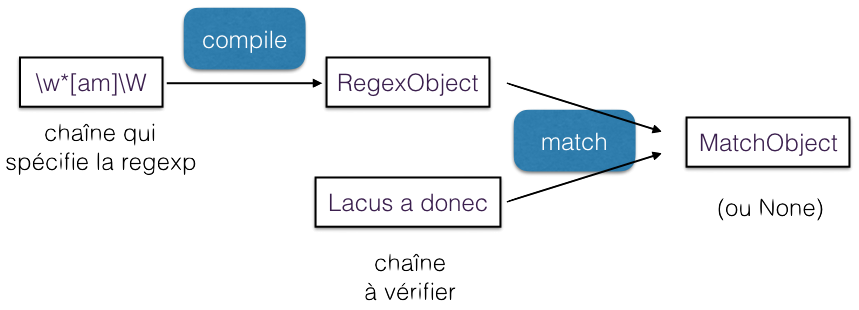
\includegraphics{medias/re-workflow.png}\\

    La méthode recommandée pour utiliser la librairie, lorsque vous avez le
même \emph{pattern} à appliquer à un grand nombre de chaînes, est de~:

\begin{itemize}
	\item 
	compiler \textbf{une seule fois} votre chaîne en un automate, qui est
	matérialisé par un objet de la classe \texttt{re.RegexObject}, en
	utilisant \texttt{re.compile},
	\item
	puis d'\textbf{utiliser directement cet
	objet} autant de fois que vous avez de chaînes.
\end{itemize}

    Nous avons utilisé dans les exemples plus haut (et nous continuerons
plus bas pour une meilleure lisibilité) des \textbf{fonctions de
commodité} du module, qui sont pratiques, par exemple, pour mettre au
point une expression régulière en mode interactif, mais qui ne
\textbf{sont pas forcément} adaptées dans tous les cas.\\

Ces fonctions de commodité fonctionnent toutes sur le même principe~:\\

\texttt{re.match(regexp,\ sample)} \(\Longleftrightarrow\)
\texttt{re.compile(regexp).match(sample)}\\

Donc à chaque fois qu'on utilise une fonction de commodité, on recompile
la chaîne en automate, ce qui, dès qu'on a plus d'une chaîne à traiter,
représente un surcoût.

    \begin{Verbatim}[commandchars=\\\{\}]
{\color{incolor}In [{\color{incolor}25}]:} \PY{c+c1}{\PYZsh{} au lieu de faire comme ci\PYZhy{}dessus:}
         
         \PY{c+c1}{\PYZsh{} imaginez 10**6 chaînes dans samples}
         \PY{k}{for} \PY{n}{sample} \PY{o+ow}{in} \PY{n}{samples}\PY{p}{:}
             \PY{n}{match} \PY{o}{=} \PY{n}{re}\PY{o}{.}\PY{n}{match}\PY{p}{(}\PY{n}{regexp3}\PY{p}{,} \PY{n}{sample}\PY{p}{)}
             \PY{n+nb}{print}\PY{p}{(}\PY{n}{f}\PY{l+s+s2}{\PYZdq{}}\PY{l+s+si}{\PYZob{}sample:\PYZgt{}16s\PYZcb{}}\PY{l+s+s2}{ → }\PY{l+s+s2}{\PYZob{}}\PY{l+s+s2}{nice(match)\PYZcb{}}\PY{l+s+s2}{\PYZdq{}}\PY{p}{)}    
\end{Verbatim}


    \begin{Verbatim}[commandchars=\\\{\}]
  890hj000nnm890 → Match!
 123abc456def789 → no
 8090abababab879 → no

    \end{Verbatim}

    \begin{Verbatim}[commandchars=\\\{\}]
{\color{incolor}In [{\color{incolor}26}]:} \PY{c+c1}{\PYZsh{} dans du vrai code on fera plutôt:}
         
         \PY{c+c1}{\PYZsh{} on compile la chaîne en automate une seule fois}
         \PY{n}{re\PYZus{}obj3} \PY{o}{=} \PY{n}{re}\PY{o}{.}\PY{n}{compile}\PY{p}{(}\PY{n}{regexp3}\PY{p}{)}
         
         \PY{c+c1}{\PYZsh{} ensuite on part directement de l\PYZsq{}automate}
         \PY{k}{for} \PY{n}{sample} \PY{o+ow}{in} \PY{n}{samples}\PY{p}{:}
             \PY{n}{match} \PY{o}{=} \PY{n}{re\PYZus{}obj3}\PY{o}{.}\PY{n}{match}\PY{p}{(}\PY{n}{sample}\PY{p}{)}
             \PY{n+nb}{print}\PY{p}{(}\PY{n}{f}\PY{l+s+s2}{\PYZdq{}}\PY{l+s+si}{\PYZob{}sample:\PYZgt{}16s\PYZcb{}}\PY{l+s+s2}{ → }\PY{l+s+s2}{\PYZob{}}\PY{l+s+s2}{nice(match)\PYZcb{}}\PY{l+s+s2}{\PYZdq{}}\PY{p}{)}
\end{Verbatim}


    \begin{Verbatim}[commandchars=\\\{\}]
  890hj000nnm890 → Match!
 123abc456def789 → no
 8090abababab879 → no

    \end{Verbatim}

    Cette deuxième version ne compile qu'une fois la chaîne en automate, et
donc est plus efficace.

    \hypertarget{les-muxe9thodes-sur-la-classe-regexobject}{%
\subparagraph{\texorpdfstring{Les méthodes sur la classe
\texttt{RegexObject}}{Les méthodes sur la classe RegexObject}}\label{les-muxe9thodes-sur-la-classe-regexobject}}

    Les objets de la classe \texttt{RegexObject} représentent donc
l'automate à état fini qui est le résultat de la compilation de
l'expression régulière. Pour résumer ce qu'on a déjà vu, les méthodes
les plus utiles sur un objet \texttt{RegexObject} sont~:

\begin{itemize}
	\item 
	\texttt{match} et \texttt{search}, qui cherchent un \emph{match} soit
	uniquement au début (\texttt{match}) ou n'importe où dans la chaîne
	(\texttt{search}),
	\item
	\texttt{findall} et \texttt{split} pour chercher
	toutes les occurences (\texttt{findall}) ou leur négatif
	(\texttt{split}),
	\item
	\texttt{sub} (qui aurait pu sans doute s'appeler
	\texttt{replace}, mais c'est comme ça) pour remplacer les occurrences de
	pattern.
\end{itemize}

    \hypertarget{exploiter-le-ruxe9sultat}{%
\subparagraph{Exploiter le résultat\\\\}\label{exploiter-le-ruxe9sultat}}

    Les \textbf{méthodes} disponibles sur la classe
\textbf{\texttt{re.MatchObject}} sont
\href{https://docs.python.org/3/library/re.html\#match-objects}{documentées
en détail ici}. On en a déjà rencontré quelques-unes, en voici à nouveau
un aperçu rapide.

    \begin{Verbatim}[commandchars=\\\{\}]
{\color{incolor}In [{\color{incolor}27}]:} \PY{c+c1}{\PYZsh{} exemple}
         \PY{n}{sample} \PY{o}{=} \PY{l+s+s2}{\PYZdq{}}\PY{l+s+s2}{    Isaac Newton, physicist}\PY{l+s+s2}{\PYZdq{}}
         \PY{n}{match} \PY{o}{=} \PY{n}{re}\PY{o}{.}\PY{n}{search}\PY{p}{(}\PY{l+s+sa}{r}\PY{l+s+s2}{\PYZdq{}}\PY{l+s+s2}{(}\PY{l+s+s2}{\PYZbs{}}\PY{l+s+s2}{w+) (?P\PYZlt{}name\PYZgt{}}\PY{l+s+s2}{\PYZbs{}}\PY{l+s+s2}{w+)}\PY{l+s+s2}{\PYZdq{}}\PY{p}{,} \PY{n}{sample}\PY{p}{)}
\end{Verbatim}


    \texttt{re} et \texttt{string} pour retrouver les données d'entrée du
match.

    \begin{Verbatim}[commandchars=\\\{\}]
{\color{incolor}In [{\color{incolor}28}]:} \PY{n}{match}\PY{o}{.}\PY{n}{string}
\end{Verbatim}


\begin{Verbatim}[commandchars=\\\{\}]
{\color{outcolor}Out[{\color{outcolor}28}]:} '    Isaac Newton, physicist'
\end{Verbatim}
            
    \begin{Verbatim}[commandchars=\\\{\}]
{\color{incolor}In [{\color{incolor}29}]:} \PY{n}{match}\PY{o}{.}\PY{n}{re}
\end{Verbatim}


\begin{Verbatim}[commandchars=\\\{\}]
{\color{outcolor}Out[{\color{outcolor}29}]:} re.compile(r'(\textbackslash{}w+) (?P<name>\textbackslash{}w+)', re.UNICODE)
\end{Verbatim}
            
    \texttt{group}, \texttt{groups}, \texttt{groupdict} pour retrouver les
morceaux de la chaîne d'entrée qui correspondent aux \textbf{groupes} de
la regexp. On peut y accéder par rang, ou par nom (comme on l'a vu plus
haut avec \texttt{needle}).

    \begin{Verbatim}[commandchars=\\\{\}]
{\color{incolor}In [{\color{incolor}30}]:} \PY{n}{match}\PY{o}{.}\PY{n}{groups}\PY{p}{(}\PY{p}{)}
\end{Verbatim}


\begin{Verbatim}[commandchars=\\\{\}]
{\color{outcolor}Out[{\color{outcolor}30}]:} ('Isaac', 'Newton')
\end{Verbatim}
            
    \begin{Verbatim}[commandchars=\\\{\}]
{\color{incolor}In [{\color{incolor}31}]:} \PY{n}{match}\PY{o}{.}\PY{n}{group}\PY{p}{(}\PY{l+m+mi}{1}\PY{p}{)}
\end{Verbatim}


\begin{Verbatim}[commandchars=\\\{\}]
{\color{outcolor}Out[{\color{outcolor}31}]:} 'Isaac'
\end{Verbatim}
            
    \begin{Verbatim}[commandchars=\\\{\}]
{\color{incolor}In [{\color{incolor}32}]:} \PY{n}{match}\PY{o}{.}\PY{n}{group}\PY{p}{(}\PY{l+s+s1}{\PYZsq{}}\PY{l+s+s1}{name}\PY{l+s+s1}{\PYZsq{}}\PY{p}{)}
\end{Verbatim}


\begin{Verbatim}[commandchars=\\\{\}]
{\color{outcolor}Out[{\color{outcolor}32}]:} 'Newton'
\end{Verbatim}
            
    \begin{Verbatim}[commandchars=\\\{\}]
{\color{incolor}In [{\color{incolor}33}]:} \PY{n}{match}\PY{o}{.}\PY{n}{group}\PY{p}{(}\PY{l+m+mi}{2}\PY{p}{)}
\end{Verbatim}


\begin{Verbatim}[commandchars=\\\{\}]
{\color{outcolor}Out[{\color{outcolor}33}]:} 'Newton'
\end{Verbatim}
            
    \begin{Verbatim}[commandchars=\\\{\}]
{\color{incolor}In [{\color{incolor}34}]:} \PY{n}{match}\PY{o}{.}\PY{n}{groupdict}\PY{p}{(}\PY{p}{)}
\end{Verbatim}


\begin{Verbatim}[commandchars=\\\{\}]
{\color{outcolor}Out[{\color{outcolor}34}]:} \{'name': 'Newton'\}
\end{Verbatim}
            
    Comme on le voit pour l'accès par rang \textbf{les indices commencent à
1} pour des raisons historiques (on peut déjà référencer
\texttt{\textbackslash{}1} en sed depuis la fin des années 70).\\

On peut aussi accéder au \textbf{groupe 0} comme étant la partie de la
chaîne de départ qui a effectivement été filtrée par l'expression
régulière, et qui peut tout à fait être au beau milieu de la chaîne de
départ, comme dans notre exemple

    \begin{Verbatim}[commandchars=\\\{\}]
{\color{incolor}In [{\color{incolor}35}]:} \PY{n}{match}\PY{o}{.}\PY{n}{group}\PY{p}{(}\PY{l+m+mi}{0}\PY{p}{)}
\end{Verbatim}


\begin{Verbatim}[commandchars=\\\{\}]
{\color{outcolor}Out[{\color{outcolor}35}]:} 'Isaac Newton'
\end{Verbatim}
            
    \texttt{expand} permet de faire une espèce de \texttt{str.format} avec
les valeurs des groupes.

    \begin{Verbatim}[commandchars=\\\{\}]
{\color{incolor}In [{\color{incolor}36}]:} \PY{n}{match}\PY{o}{.}\PY{n}{expand}\PY{p}{(}\PY{l+s+sa}{r}\PY{l+s+s2}{\PYZdq{}}\PY{l+s+s2}{last\PYZus{}name }\PY{l+s+s2}{\PYZbs{}}\PY{l+s+s2}{g\PYZlt{}name\PYZgt{} first\PYZus{}name }\PY{l+s+s2}{\PYZbs{}}\PY{l+s+s2}{1}\PY{l+s+s2}{\PYZdq{}}\PY{p}{)}
\end{Verbatim}


\begin{Verbatim}[commandchars=\\\{\}]
{\color{outcolor}Out[{\color{outcolor}36}]:} 'last\_name Newton first\_name Isaac'
\end{Verbatim}
            
    \texttt{span} pour connaître les index dans la chaîne d'entrée pour un
groupe donné.

    \begin{Verbatim}[commandchars=\\\{\}]
{\color{incolor}In [{\color{incolor}37}]:} \PY{n}{begin}\PY{p}{,} \PY{n}{end} \PY{o}{=} \PY{n}{match}\PY{o}{.}\PY{n}{span}\PY{p}{(}\PY{l+s+s1}{\PYZsq{}}\PY{l+s+s1}{name}\PY{l+s+s1}{\PYZsq{}}\PY{p}{)}
         \PY{n}{sample}\PY{p}{[}\PY{n}{begin}\PY{p}{:}\PY{n}{end}\PY{p}{]}
\end{Verbatim}


\begin{Verbatim}[commandchars=\\\{\}]
{\color{outcolor}Out[{\color{outcolor}37}]:} 'Newton'
\end{Verbatim}
            
    \hypertarget{les-diffuxe9rents-modes-flags}{%
\subparagraph{\texorpdfstring{Les différents modes
(\emph{flags})}{Les différents modes (flags)}}\label{les-diffuxe9rents-modes-flags}}

    Enfin il faut noter qu'on peut passer à \texttt{re.compile} un certain
nombre de \emph{flags} qui modifient globalement l'interprétation de la
chaîne, et qui peuvent rendre service.\\

    Vous trouverez
\href{https://docs.python.org/3/library/re.html\#module-contents}{une
liste exhaustive de ces \emph{flags} ici}. Ils ont en général un nom
long et parlant, et un alias court sur un seul caractère. Les plus
utiles sont sans doute~:

\begin{itemize}
	\item 
	\texttt{IGNORECASE} (\emph{alias} \texttt{I})
	pour, eh bien, ne pas faire la différence entre minuscules et
	majuscules,
	\item
	\texttt{UNICODE} (\emph{alias} \texttt{U}) pour rendre les
	séquences \texttt{\textbackslash{}w} et autres basées sur les propriétés
	des caractères dans la norme Unicode,
	\item
	\texttt{LOCALE} (\emph{alias}
	\texttt{L}) cette fois \texttt{\textbackslash{}w} dépend du
	\texttt{locale} courant,
	\item
	\texttt{MULTILINE} (\emph{alias} \texttt{M}), et
	\item
	\texttt{DOTALL} (\emph{alias} S) pour ces deux flags voir la
	discussion à la fin du complément.
\end{itemize}

    Comme c'est souvent le cas, on doit passer à \texttt{re.compile} un
\textbf{ou logique} (caractère \texttt{\textbar{}}) des différents flags
que l'on veut utiliser, c'est-à-dire qu'on fera par exemple

    \begin{Verbatim}[commandchars=\\\{\}]
{\color{incolor}In [{\color{incolor}38}]:} \PY{n}{regexp} \PY{o}{=} \PY{l+s+s2}{\PYZdq{}}\PY{l+s+s2}{a*b+}\PY{l+s+s2}{\PYZdq{}}
         \PY{n}{re\PYZus{}obj} \PY{o}{=} \PY{n}{re}\PY{o}{.}\PY{n}{compile}\PY{p}{(}\PY{n}{regexp}\PY{p}{,} \PY{n}{flags}\PY{o}{=}\PY{n}{re}\PY{o}{.}\PY{n}{IGNORECASE} \PY{o}{|} \PY{n}{re}\PY{o}{.}\PY{n}{DEBUG}\PY{p}{)}
\end{Verbatim}


    \begin{Verbatim}[commandchars=\\\{\}]
MAX\_REPEAT 0 MAXREPEAT
  LITERAL 97
MAX\_REPEAT 1 MAXREPEAT
  LITERAL 98

    \end{Verbatim}

    \begin{Verbatim}[commandchars=\\\{\}]
{\color{incolor}In [{\color{incolor}39}]:} \PY{c+c1}{\PYZsh{} on ignore la casse des caractères }
         \PY{n+nb}{print}\PY{p}{(}\PY{n}{regexp}\PY{p}{,} \PY{l+s+s2}{\PYZdq{}}\PY{l+s+s2}{\PYZhy{}\PYZgt{}}\PY{l+s+s2}{\PYZdq{}}\PY{p}{,} \PY{n}{nice}\PY{p}{(}\PY{n}{re\PYZus{}obj}\PY{o}{.}\PY{n}{match}\PY{p}{(}\PY{l+s+s2}{\PYZdq{}}\PY{l+s+s2}{AabB}\PY{l+s+s2}{\PYZdq{}}\PY{p}{)}\PY{p}{)}\PY{p}{)}
\end{Verbatim}


    \begin{Verbatim}[commandchars=\\\{\}]
a*b+ -> Match!

    \end{Verbatim}

    \hypertarget{comment-construire-une-expression-ruxe9guliuxe8re}{%
\subsubsection{Comment construire une expression
régulière}\label{comment-construire-une-expression-ruxe9guliuxe8re}}

    Nous pouvons à présent voir comment construire une expression régulière,
en essayant de rester synthétique (la
\href{https://docs.python.org/3/library/re.html}{documentation du module
\texttt{re}} en donne une version exhaustive).

    \hypertarget{la-brique-de-base-le-caractuxe8re}{%
\subparagraph{La brique de base : le
caractère\\\\}\label{la-brique-de-base-le-caractuxe8re}}

    Au commencement il faut spécifier des caractères.

\begin{itemize}
	\item 
    \textbf{un seul} caractère:
    \begin{itemize}
    	\item 
		vous le citez tel quel, en le précédent d'un backslash
		\texttt{\textbackslash{}} s'il a par ailleurs un sens spécial dans le
		micro-langage de regexps (comme \texttt{+}, \texttt{*}, \texttt{{[}},
		etc.);
	\end{itemize}
	\item	
	l'\textbf{attrape-tout} (\emph{wildcard}):
	\begin{itemize}
		\item 
		un point \texttt{.} signifie ``n'importe quel caractère'';
	\end{itemize}
	\item	
	\textbf{un ensemble}
	de caractères avec la notation \texttt{{[}...{]}} qui permet de décrire
	par exemple:
	\begin{itemize}
		\item 
		\texttt{{[}a1={]}} un ensemble in extenso, ici un
		caractère parmi \texttt{a}, \texttt{1}, ou \texttt{=},
		\item
		\texttt{{[}a-z{]}} un intervalle de caractères, ici de \texttt{a} à
		\texttt{z},
		\item
		\texttt{{[}15e-g{]}} un mélange des deux, ici un ensemble
		qui contiendrait \texttt{1}, \texttt{5}, \texttt{e}, \texttt{f} et
		\texttt{g},
		\item 	
		\texttt{{[}\^{}15e-g{]}} une \textbf{négation}, qui a
		\texttt{\^{}} comme premier caractère dans les \texttt{{[}{]}}, ici tout
		sauf l'ensemble précédent;
	\end{itemize}	
	\item
	un \textbf{ensemble prédéfini} de
	caractères, qui peuvent alors dépendre de l'environnement (UNICODE et
	LOCALE) avec entre autres les notations:
	\begin{itemize}
		\item 
		\texttt{\textbackslash{}w}
		les caractères alphanumériques, et \texttt{\textbackslash{}W} (les
		autres),
		\item
		\texttt{\textbackslash{}s} les caractères ``blancs'' -
		espace, tabulation, saut de ligne, etc., et \texttt{\textbackslash{}S}
		(les autres),
		\item
		\texttt{\textbackslash{}d} pour les chiffres, et
		\texttt{\textbackslash{}D} (les autres).
	\end{itemize}		
\end{itemize}

    \begin{Verbatim}[commandchars=\\\{\}]
{\color{incolor}In [{\color{incolor}40}]:} \PY{n}{sample} \PY{o}{=} \PY{l+s+s2}{\PYZdq{}}\PY{l+s+s2}{abcd}\PY{l+s+s2}{\PYZdq{}}
         
         \PY{k}{for} \PY{n}{regexp} \PY{o+ow}{in} \PY{p}{[}\PY{l+s+s1}{\PYZsq{}}\PY{l+s+s1}{abcd}\PY{l+s+s1}{\PYZsq{}}\PY{p}{,} \PY{l+s+s1}{\PYZsq{}}\PY{l+s+s1}{ab[cd][cd]}\PY{l+s+s1}{\PYZsq{}}\PY{p}{,} \PY{l+s+s1}{\PYZsq{}}\PY{l+s+s1}{ab[a\PYZhy{}z]d}\PY{l+s+s1}{\PYZsq{}}\PY{p}{,} \PY{l+s+sa}{r}\PY{l+s+s1}{\PYZsq{}}\PY{l+s+s1}{abc.}\PY{l+s+s1}{\PYZsq{}}\PY{p}{,} \PY{l+s+sa}{r}\PY{l+s+s1}{\PYZsq{}}\PY{l+s+s1}{abc}\PY{l+s+s1}{\PYZbs{}}\PY{l+s+s1}{.}\PY{l+s+s1}{\PYZsq{}}\PY{p}{]}\PY{p}{:}
             \PY{n}{match} \PY{o}{=} \PY{n}{re}\PY{o}{.}\PY{n}{match}\PY{p}{(}\PY{n}{regexp}\PY{p}{,} \PY{n}{sample}\PY{p}{)}
             \PY{n+nb}{print}\PY{p}{(}\PY{n}{f}\PY{l+s+s2}{\PYZdq{}}\PY{l+s+si}{\PYZob{}sample\PYZcb{}}\PY{l+s+s2}{ / }\PY{l+s+si}{\PYZob{}regexp:\PYZlt{}10s\PYZcb{}}\PY{l+s+s2}{ → }\PY{l+s+s2}{\PYZob{}}\PY{l+s+s2}{nice(match)\PYZcb{}}\PY{l+s+s2}{\PYZdq{}}\PY{p}{)}
\end{Verbatim}


    \begin{Verbatim}[commandchars=\\\{\}]
abcd / abcd       → Match!
abcd / ab[cd][cd] → Match!
abcd / ab[a-z]d   → Match!
abcd / abc.       → Match!
abcd / abc\textbackslash{}.      → no

    \end{Verbatim}

    Pour ce dernier exemple, comme on a backslashé le \texttt{.} il faut que
la chaîne en entrée contienne vraiment un \texttt{.}

    \begin{Verbatim}[commandchars=\\\{\}]
{\color{incolor}In [{\color{incolor}41}]:} \PY{n+nb}{print}\PY{p}{(}\PY{n}{nice}\PY{p}{(}\PY{n}{re}\PY{o}{.}\PY{n}{match} \PY{p}{(}\PY{l+s+sa}{r}\PY{l+s+s2}{\PYZdq{}}\PY{l+s+s2}{abc}\PY{l+s+s2}{\PYZbs{}}\PY{l+s+s2}{.}\PY{l+s+s2}{\PYZdq{}}\PY{p}{,} \PY{l+s+s2}{\PYZdq{}}\PY{l+s+s2}{abc.}\PY{l+s+s2}{\PYZdq{}}\PY{p}{)}\PY{p}{)}\PY{p}{)}
\end{Verbatim}


    \begin{Verbatim}[commandchars=\\\{\}]
Match!

    \end{Verbatim}

    \hypertarget{en-suxe9rie-ou-en-paralluxe8le}{%
\subparagraph{En série ou en
parallèle}\label{en-suxe9rie-ou-en-paralluxe8le}}

    Si je fais une analogie avec les montages électriques, jusqu'ici on a vu
le montage en série, on met des expressions régulières bout à bout qui
filtrent (\texttt{match}) la chaine en entrée séquentiellement du début
à la fin. On a \emph{un peu} de marge pour spécifier des alternatives,
lorsqu'on fait par exemple

\begin{verbatim}
"ab[cd]ef"
\end{verbatim}

mais c'est limité à \textbf{un seul} caractère. Si on veut reconnaitre
deux mots qui n'ont pas grand-chose à voir comme \texttt{abc}
\textbf{ou} \texttt{def}, il faut en quelque sorte mettre deux regexps
en parallèle, et c'est ce que permet l'opérateur \texttt{\textbar{}}

    \begin{Verbatim}[commandchars=\\\{\}]
{\color{incolor}In [{\color{incolor}42}]:} \PY{n}{regexp} \PY{o}{=} \PY{l+s+s2}{\PYZdq{}}\PY{l+s+s2}{abc|def}\PY{l+s+s2}{\PYZdq{}}
         
         \PY{k}{for} \PY{n}{sample} \PY{o+ow}{in} \PY{p}{[}\PY{l+s+s1}{\PYZsq{}}\PY{l+s+s1}{abc}\PY{l+s+s1}{\PYZsq{}}\PY{p}{,} \PY{l+s+s1}{\PYZsq{}}\PY{l+s+s1}{def}\PY{l+s+s1}{\PYZsq{}}\PY{p}{,} \PY{l+s+s1}{\PYZsq{}}\PY{l+s+s1}{aef}\PY{l+s+s1}{\PYZsq{}}\PY{p}{]}\PY{p}{:}
             \PY{n}{match} \PY{o}{=} \PY{n}{re}\PY{o}{.}\PY{n}{match}\PY{p}{(}\PY{n}{regexp}\PY{p}{,} \PY{n}{sample}\PY{p}{)}
             \PY{n+nb}{print}\PY{p}{(}\PY{n}{f}\PY{l+s+s2}{\PYZdq{}}\PY{l+s+si}{\PYZob{}sample\PYZcb{}}\PY{l+s+s2}{ / }\PY{l+s+si}{\PYZob{}regexp\PYZcb{}}\PY{l+s+s2}{ → }\PY{l+s+s2}{\PYZob{}}\PY{l+s+s2}{nice(match)\PYZcb{}}\PY{l+s+s2}{\PYZdq{}}\PY{p}{)}
\end{Verbatim}


    \begin{Verbatim}[commandchars=\\\{\}]
abc / abc|def → Match!
def / abc|def → Match!
aef / abc|def → no

    \end{Verbatim}

    \hypertarget{fins-de-chauxeene}{%
\subparagraph{Fin(s) de chaîne\\\\}\label{fins-de-chauxeene}}

    Selon que vous utilisez \texttt{match} ou \texttt{search}, vous précisez
si vous vous intéressez uniquement à un match en début (\texttt{match})
ou n'importe où (\texttt{search}) dans la chaîne.\\

Mais indépendamment de cela, il peut être intéressant de ``coller''
l'expression en début ou en fin de ligne, et pour ça il existe des
caractères spéciaux:

\begin{itemize}
	\item
	\texttt{\^{}} lorsqu'il est utilisé comme un
	caractère (c'est à dire pas en début de \texttt{{[}{]}}) signifie un
	début de chaîne;
	\item
	\texttt{\textbackslash{}A} a le même sens (sauf en
	mode MULTILINE), et je le recommande de préférence à \texttt{\^{}} qui
	est déjà pas mal surchargé;
	\item
	\texttt{\$} matche une fin de ligne;
	\item
	\texttt{\textbackslash{}Z} est voisin mais pas tout à fait identique.
\end{itemize}

Reportez-vous à la documentation pour le détails des différences.
Attention aussi à entrer le \texttt{\^{}} correctement, il vous faut le
caractère ASCII et non un voisin dans la ménagerie Unicode.

    \begin{Verbatim}[commandchars=\\\{\}]
{\color{incolor}In [{\color{incolor}43}]:} \PY{n}{sample} \PY{o}{=} \PY{l+s+s1}{\PYZsq{}}\PY{l+s+s1}{abcd}\PY{l+s+s1}{\PYZsq{}}
         
         \PY{k}{for} \PY{n}{regexp} \PY{o+ow}{in} \PY{p}{[} \PY{l+s+sa}{r}\PY{l+s+s1}{\PYZsq{}}\PY{l+s+s1}{bc}\PY{l+s+s1}{\PYZsq{}}\PY{p}{,} \PY{l+s+sa}{r}\PY{l+s+s1}{\PYZsq{}}\PY{l+s+s1}{\PYZbs{}}\PY{l+s+s1}{Aabc}\PY{l+s+s1}{\PYZsq{}}\PY{p}{,} \PY{l+s+sa}{r}\PY{l+s+s1}{\PYZsq{}}\PY{l+s+s1}{\PYZca{}abc}\PY{l+s+s1}{\PYZsq{}}\PY{p}{,} 
                         \PY{l+s+sa}{r}\PY{l+s+s1}{\PYZsq{}}\PY{l+s+s1}{\PYZbs{}}\PY{l+s+s1}{Abc}\PY{l+s+s1}{\PYZsq{}}\PY{p}{,} \PY{l+s+sa}{r}\PY{l+s+s1}{\PYZsq{}}\PY{l+s+s1}{\PYZca{}bc}\PY{l+s+s1}{\PYZsq{}}\PY{p}{,} \PY{l+s+sa}{r}\PY{l+s+s1}{\PYZsq{}}\PY{l+s+s1}{bcd}\PY{l+s+s1}{\PYZbs{}}\PY{l+s+s1}{Z}\PY{l+s+s1}{\PYZsq{}}\PY{p}{,} 
                         \PY{l+s+sa}{r}\PY{l+s+s1}{\PYZsq{}}\PY{l+s+s1}{bcd\PYZdl{}}\PY{l+s+s1}{\PYZsq{}}\PY{p}{,} \PY{l+s+sa}{r}\PY{l+s+s1}{\PYZsq{}}\PY{l+s+s1}{bc}\PY{l+s+s1}{\PYZbs{}}\PY{l+s+s1}{Z}\PY{l+s+s1}{\PYZsq{}}\PY{p}{,} \PY{l+s+sa}{r}\PY{l+s+s1}{\PYZsq{}}\PY{l+s+s1}{bc\PYZdl{}}\PY{l+s+s1}{\PYZsq{}} \PY{p}{]}\PY{p}{:}
             \PY{n}{match} \PY{o}{=} \PY{n}{re}\PY{o}{.}\PY{n}{match}\PY{p}{(}\PY{n}{regexp}\PY{p}{,} \PY{n}{sample}\PY{p}{)}
             \PY{n}{search} \PY{o}{=} \PY{n}{re}\PY{o}{.}\PY{n}{search}\PY{p}{(}\PY{n}{regexp}\PY{p}{,} \PY{n}{sample}\PY{p}{)}
             \PY{n+nb}{print}\PY{p}{(}\PY{n}{f}\PY{l+s+s2}{\PYZdq{}}\PY{l+s+si}{\PYZob{}sample\PYZcb{}}\PY{l+s+s2}{ / }\PY{l+s+si}{\PYZob{}regexp:5s\PYZcb{}}\PY{l+s+s2}{ match → }\PY{l+s+s2}{\PYZob{}}\PY{l+s+s2}{nice(match):6s\PYZcb{} search → }\PY{l+s+s2}{\PYZob{}}\PY{l+s+s2}{nice(search)\PYZcb{}}\PY{l+s+s2}{\PYZdq{}}\PY{p}{)}
\end{Verbatim}


    \begin{Verbatim}[commandchars=\\\{\}]
abcd / bc    match → no     search → Match!
abcd / \textbackslash{}Aabc match → Match! search → Match!
abcd / \^{}abc  match → Match! search → Match!
abcd / \textbackslash{}Abc  match → no     search → no
abcd / \^{}bc   match → no     search → no
abcd / bcd\textbackslash{}Z match → no     search → Match!
abcd / bcd\$  match → no     search → Match!
abcd / bc\textbackslash{}Z  match → no     search → no
abcd / bc\$   match → no     search → no

    \end{Verbatim}

    On a en effet bien le pattern \texttt{bc} dans la chaine en entrée, mais
il n'est ni au début ni à la fin.

    \hypertarget{parenthuxe9ser---grouper}{%
\subparagraph{Parenthéser - (grouper)\\\\}\label{parenthuxe9ser---grouper}}

    Pour pouvoir faire des montages élaborés, il faut pouvoir parenthéser.

    \begin{Verbatim}[commandchars=\\\{\}]
{\color{incolor}In [{\color{incolor}44}]:} \PY{c+c1}{\PYZsh{} une parenthése dans une RE }
         \PY{c+c1}{\PYZsh{} pour mettre en ligne:}
         \PY{c+c1}{\PYZsh{} un début \PYZsq{}a\PYZsq{}, }
         \PY{c+c1}{\PYZsh{} un milieu \PYZsq{}bc\PYZsq{} ou \PYZsq{}de\PYZsq{} }
         \PY{c+c1}{\PYZsh{} et une fin \PYZsq{}f\PYZsq{}}
         \PY{n}{regexp} \PY{o}{=} \PY{l+s+s2}{\PYZdq{}}\PY{l+s+s2}{a(bc|de)f}\PY{l+s+s2}{\PYZdq{}}
\end{Verbatim}

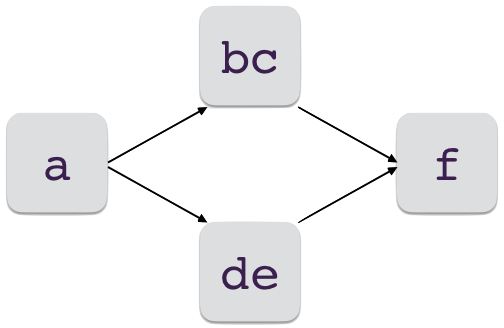
\includegraphics{medias/re-serie-parallele.png}\\
    

    \begin{Verbatim}[commandchars=\\\{\}]
{\color{incolor}In [{\color{incolor}45}]:} \PY{k}{for} \PY{n}{sample} \PY{o+ow}{in} \PY{p}{[}\PY{l+s+s1}{\PYZsq{}}\PY{l+s+s1}{abcf}\PY{l+s+s1}{\PYZsq{}}\PY{p}{,} \PY{l+s+s1}{\PYZsq{}}\PY{l+s+s1}{adef}\PY{l+s+s1}{\PYZsq{}}\PY{p}{,}  \PY{l+s+s1}{\PYZsq{}}\PY{l+s+s1}{abef}\PY{l+s+s1}{\PYZsq{}}\PY{p}{,} \PY{l+s+s1}{\PYZsq{}}\PY{l+s+s1}{abf}\PY{l+s+s1}{\PYZsq{}}\PY{p}{]}\PY{p}{:}
             \PY{n}{match} \PY{o}{=} \PY{n}{re}\PY{o}{.}\PY{n}{match}\PY{p}{(}\PY{n}{regexp}\PY{p}{,} \PY{n}{sample}\PY{p}{)}
             \PY{n+nb}{print}\PY{p}{(}\PY{n}{f}\PY{l+s+s2}{\PYZdq{}}\PY{l+s+si}{\PYZob{}sample:\PYZgt{}4s\PYZcb{}}\PY{l+s+s2}{ → }\PY{l+s+s2}{\PYZob{}}\PY{l+s+s2}{nice(match)\PYZcb{}}\PY{l+s+s2}{\PYZdq{}}\PY{p}{)}
\end{Verbatim}


    \begin{Verbatim}[commandchars=\\\{\}]
abcf → Match!
adef → Match!
abef → no
 abf → no

    \end{Verbatim}

    Les parenthèses jouent un rôle additionel de \textbf{groupe}, ce qui
signifie qu'on \textbf{peut retrouver} le texte correspondant à
l'expression régulière comprise dans les \texttt{()}. Par exemple, pour
le premier match

    \begin{Verbatim}[commandchars=\\\{\}]
{\color{incolor}In [{\color{incolor}46}]:} \PY{n}{sample} \PY{o}{=} \PY{l+s+s1}{\PYZsq{}}\PY{l+s+s1}{abcf}\PY{l+s+s1}{\PYZsq{}}
         \PY{n}{match} \PY{o}{=} \PY{n}{re}\PY{o}{.}\PY{n}{match}\PY{p}{(}\PY{n}{regexp}\PY{p}{,} \PY{n}{sample}\PY{p}{)}
         \PY{n+nb}{print}\PY{p}{(}\PY{n}{f}\PY{l+s+s2}{\PYZdq{}}\PY{l+s+si}{\PYZob{}sample\PYZcb{}}\PY{l+s+s2}{, }\PY{l+s+si}{\PYZob{}regexp\PYZcb{}}\PY{l+s+s2}{ → }\PY{l+s+s2}{\PYZob{}}\PY{l+s+s2}{match.groups()\PYZcb{}}\PY{l+s+s2}{\PYZdq{}}\PY{p}{)}
\end{Verbatim}


    \begin{Verbatim}[commandchars=\\\{\}]
abcf, a(bc|de)f → ('bc',)

    \end{Verbatim}

    dans cet exemple, on n'a utilisé qu'un seul groupe \texttt{()}, et le
morceau de chaîne qui correspond à ce groupe se trouve donc être le seul
groupe retourné par \texttt{MatchObject.group}.

    \hypertarget{compter-les-ruxe9puxe9titions}{%
\subparagraph{Compter les
répétitions\\\\}\label{compter-les-ruxe9puxe9titions}}

    Vous disposez des opérateurs suivants~:
    
\begin{itemize}
	\item 
   	\texttt{*} l'étoile qui
	signifie n'importe quel nombre, même nul, d'occurrences - par exemple,
	\texttt{(ab)*} pour indiquer
	\texttt{\textquotesingle{}\textquotesingle{}} ou
	\texttt{\textquotesingle{}ab\textquotesingle{}} ou
	\texttt{\textquotesingle{}abab\textquotesingle{}} ou etc.,
	\item
	\texttt{+}
	le plus qui signifie au moins une occurrence - e.g. \texttt{(ab)+} pour
	\texttt{ab} ou \texttt{abab} ou \texttt{ababab} ou etc,
	\item
	\texttt{?} qui
	indique une option, c'est-à-dire 0 ou 1 occurence - autrement dit
	\texttt{(ab)?} matche \texttt{\textquotesingle{}\textquotesingle{}} ou
	\texttt{ab},
	\item
	\texttt{\{n\}} pour exactement n occurrences de
	\texttt{(ab)} - e.g. \texttt{(ab)\{3\}} qui serait exactement équivalent
	à \texttt{ababab},
	\item
	\texttt{\{m,n\}} entre m et n fois inclusivement.
\end{itemize}

    \begin{Verbatim}[commandchars=\\\{\}]
{\color{incolor}In [{\color{incolor}47}]:} \PY{n}{samples} \PY{o}{=} \PY{p}{[}\PY{n}{n}\PY{o}{*}\PY{l+s+s1}{\PYZsq{}}\PY{l+s+s1}{ab}\PY{l+s+s1}{\PYZsq{}} \PY{k}{for} \PY{n}{n} \PY{o+ow}{in} \PY{p}{[}\PY{l+m+mi}{0}\PY{p}{,} \PY{l+m+mi}{1}\PY{p}{,} \PY{l+m+mi}{3}\PY{p}{,} \PY{l+m+mi}{4}\PY{p}{]}\PY{p}{]} \PY{o}{+} \PY{p}{[}\PY{l+s+s1}{\PYZsq{}}\PY{l+s+s1}{baba}\PY{l+s+s1}{\PYZsq{}}\PY{p}{]}
         
         \PY{k}{for} \PY{n}{regexp} \PY{o+ow}{in} \PY{p}{[}\PY{l+s+s1}{\PYZsq{}}\PY{l+s+s1}{(ab)*}\PY{l+s+s1}{\PYZsq{}}\PY{p}{,} \PY{l+s+s1}{\PYZsq{}}\PY{l+s+s1}{(ab)+}\PY{l+s+s1}{\PYZsq{}}\PY{p}{,} \PY{l+s+s1}{\PYZsq{}}\PY{l+s+s1}{(ab)}\PY{l+s+si}{\PYZob{}3\PYZcb{}}\PY{l+s+s1}{\PYZsq{}}\PY{p}{,} \PY{l+s+s1}{\PYZsq{}}\PY{l+s+s1}{(ab)}\PY{l+s+s1}{\PYZob{}}\PY{l+s+s1}{3,4\PYZcb{}}\PY{l+s+s1}{\PYZsq{}}\PY{p}{]}\PY{p}{:}
             \PY{c+c1}{\PYZsh{} on ajoute \PYZbs{}A \PYZbs{}Z pour matcher toute la chaine}
             \PY{n}{line\PYZus{}regexp} \PY{o}{=} \PY{l+s+sa}{r}\PY{l+s+s2}{\PYZdq{}}\PY{l+s+s2}{\PYZbs{}}\PY{l+s+s2}{A}\PY{l+s+si}{\PYZob{}\PYZcb{}}\PY{l+s+s2}{\PYZbs{}}\PY{l+s+s2}{Z}\PY{l+s+s2}{\PYZdq{}}\PY{o}{.}\PY{n}{format}\PY{p}{(}\PY{n}{regexp}\PY{p}{)}
             \PY{k}{for} \PY{n}{sample} \PY{o+ow}{in} \PY{n}{samples}\PY{p}{:}
                 \PY{n}{match} \PY{o}{=} \PY{n}{re}\PY{o}{.}\PY{n}{match}\PY{p}{(}\PY{n}{line\PYZus{}regexp}\PY{p}{,} \PY{n}{sample}\PY{p}{)}
                 \PY{n+nb}{print}\PY{p}{(}\PY{n}{f}\PY{l+s+s2}{\PYZdq{}}\PY{l+s+si}{\PYZob{}sample:\PYZgt{}8s\PYZcb{}}\PY{l+s+s2}{ / }\PY{l+s+si}{\PYZob{}line\PYZus{}regexp:14s\PYZcb{}}\PY{l+s+s2}{ → }\PY{l+s+s2}{\PYZob{}}\PY{l+s+s2}{nice(match)\PYZcb{}}\PY{l+s+s2}{\PYZdq{}}\PY{p}{)}
\end{Verbatim}


    \begin{Verbatim}[commandchars=\\\{\}]
         / \textbackslash{}A(ab)*\textbackslash{}Z      → Match!
      ab / \textbackslash{}A(ab)*\textbackslash{}Z      → Match!
  ababab / \textbackslash{}A(ab)*\textbackslash{}Z      → Match!
abababab / \textbackslash{}A(ab)*\textbackslash{}Z      → Match!
    baba / \textbackslash{}A(ab)*\textbackslash{}Z      → no
         / \textbackslash{}A(ab)+\textbackslash{}Z      → no
      ab / \textbackslash{}A(ab)+\textbackslash{}Z      → Match!
  ababab / \textbackslash{}A(ab)+\textbackslash{}Z      → Match!
abababab / \textbackslash{}A(ab)+\textbackslash{}Z      → Match!
    baba / \textbackslash{}A(ab)+\textbackslash{}Z      → no
         / \textbackslash{}A(ab)\{3\}\textbackslash{}Z    → no
      ab / \textbackslash{}A(ab)\{3\}\textbackslash{}Z    → no
  ababab / \textbackslash{}A(ab)\{3\}\textbackslash{}Z    → Match!
abababab / \textbackslash{}A(ab)\{3\}\textbackslash{}Z    → no
    baba / \textbackslash{}A(ab)\{3\}\textbackslash{}Z    → no
         / \textbackslash{}A(ab)\{3,4\}\textbackslash{}Z  → no
      ab / \textbackslash{}A(ab)\{3,4\}\textbackslash{}Z  → no
  ababab / \textbackslash{}A(ab)\{3,4\}\textbackslash{}Z  → Match!
abababab / \textbackslash{}A(ab)\{3,4\}\textbackslash{}Z  → Match!
    baba / \textbackslash{}A(ab)\{3,4\}\textbackslash{}Z  → no

    \end{Verbatim}

    \hypertarget{groupes-et-contraintes}{%
\subparagraph{Groupes et contraintes\\\\}\label{groupes-et-contraintes}}

    Nous avons déjà vu un exemple de groupe nommé (voir \texttt{needle} plus
haut), les opérateurs que l'on peut citer dans cette catégorie sont~:

\begin{itemize}
	\item 
	\texttt{(...)} les parenthèses définissent un groupe anonyme,
	\item
	\texttt{(?P\textless{}name\textgreater{}...)} définit un groupe nommé,
	\item
	\texttt{(?:...)} permet de mettre des parenthèses mais sans créer un
	groupe, pour optimiser l'exécution puisqu'on n'a pas besoin de conserver
	les liens vers la chaîne d'entrée,
	\item
	\texttt{(?P=name)} qui ne matche
	que si l'on retrouve à cet endroit de l'entrée la même sous-chaîne que
	celle trouvée pour le groupe \texttt{name} en amont,
	\item
	enfin
	\texttt{(?=...)}, \texttt{(?!...)}et \texttt{(?\textless{}=...)}
	permettent des contraintes encore plus élaborées, nous vous laissons le
	soin d'expérimenter avec elles si vous êtes intéressés; sachez toutefois
	que l'utilisation de telles constructions peut en théorie rendre
	l'interprétation de votre expression régulière beaucoup moins efficace.
\end{itemize}

    \hypertarget{greedy-vs-non-greedy}{%
\subparagraph{\texorpdfstring{Greedy \emph{vs}
non-greedy}{Greedy vs non-greedy}\\\\}\label{greedy-vs-non-greedy}}

    Lorsqu'on stipule une répétition un nombre indéfini de fois, il se peut
qu'il existe \textbf{plusieurs} façons de filtrer l'entrée avec
l'expression régulière. Que ce soit avec \texttt{*}, ou \texttt{+}, ou
\texttt{?}, l'algorithme va toujours essayer de trouver la
\textbf{séquence la plus longue}, c'est pourquoi on qualifie l'approche
de \emph{greedy} - quelque chose comme glouton en français.

    \begin{Verbatim}[commandchars=\\\{\}]
{\color{incolor}In [{\color{incolor}48}]:} \PY{c+c1}{\PYZsh{} un fragment d\PYZsq{}HTML }
         \PY{n}{line}\PY{o}{=}\PY{l+s+s1}{\PYZsq{}}\PY{l+s+s1}{\PYZlt{}h1\PYZgt{}Title\PYZlt{}/h1\PYZgt{}}\PY{l+s+s1}{\PYZsq{}}
         
         \PY{c+c1}{\PYZsh{} si on cherche un texte quelconque entre crochets}
         \PY{c+c1}{\PYZsh{} c\PYZsq{}est\PYZhy{}à\PYZhy{}dire l\PYZsq{}expression régulière \PYZdq{}\PYZlt{}.*\PYZgt{}\PYZdq{}}
         \PY{n}{re\PYZus{}greedy} \PY{o}{=} \PY{l+s+s1}{\PYZsq{}}\PY{l+s+s1}{\PYZlt{}.*\PYZgt{}}\PY{l+s+s1}{\PYZsq{}}
         
         \PY{c+c1}{\PYZsh{} on obtient ceci}
         \PY{c+c1}{\PYZsh{} on rappelle que group(0) montre la partie du fragment}
         \PY{c+c1}{\PYZsh{} HTML qui matche l\PYZsq{}expression régulière}
         \PY{n}{match} \PY{o}{=} \PY{n}{re}\PY{o}{.}\PY{n}{match}\PY{p}{(}\PY{n}{re\PYZus{}greedy}\PY{p}{,} \PY{n}{line}\PY{p}{)}
         \PY{n}{match}\PY{o}{.}\PY{n}{group}\PY{p}{(}\PY{l+m+mi}{0}\PY{p}{)}
\end{Verbatim}


\begin{Verbatim}[commandchars=\\\{\}]
{\color{outcolor}Out[{\color{outcolor}48}]:} '<h1>Title</h1>'
\end{Verbatim}
            
    Ça n'est pas forcément ce qu'on voulait faire, aussi on peut spécifier
l'approche inverse, c'est-à-dire de trouver la \textbf{plus-petite}
chaîne qui matche, dans une approche dite \emph{non-greedy}, avec les
opérateurs suivants~:

\begin{itemize}
	\item 
	\texttt{*?} : \texttt{*} mais \emph{non-greedy},
	\item
	\texttt{+?} : \texttt{+} mais \emph{non-greedy},
	\item 
	\texttt{??} : \texttt{?} mais \emph{non-greedy},
\end{itemize}

    \begin{Verbatim}[commandchars=\\\{\}]
{\color{incolor}In [{\color{incolor}49}]:} \PY{c+c1}{\PYZsh{} ici on va remplacer * par *? pour rendre l\PYZsq{}opérateur * non\PYZhy{}greedy}
         \PY{n}{re\PYZus{}non\PYZus{}greedy} \PY{o}{=} \PY{n}{re\PYZus{}greedy} \PY{o}{=} \PY{l+s+s1}{\PYZsq{}}\PY{l+s+s1}{\PYZlt{}.*?\PYZgt{}}\PY{l+s+s1}{\PYZsq{}}
         
         \PY{c+c1}{\PYZsh{} mais on continue à cherche un texte entre \PYZlt{}\PYZgt{} naturellement}
         \PY{c+c1}{\PYZsh{} si bien que cette fois, on obtient}
         \PY{n}{match} \PY{o}{=} \PY{n}{re}\PY{o}{.}\PY{n}{match}\PY{p}{(}\PY{n}{re\PYZus{}non\PYZus{}greedy}\PY{p}{,} \PY{n}{line}\PY{p}{)}
         \PY{n}{match}\PY{o}{.}\PY{n}{group}\PY{p}{(}\PY{l+m+mi}{0}\PY{p}{)}
\end{Verbatim}


\begin{Verbatim}[commandchars=\\\{\}]
{\color{outcolor}Out[{\color{outcolor}49}]:} '<h1>'
\end{Verbatim}
            
    \hypertarget{sagissant-du-traitement-des-fins-de-ligne}{%
\subparagraph{S'agissant du traitement des fins de
ligne\\\\}\label{sagissant-du-traitement-des-fins-de-ligne}}

    Il peut être utile, pour conclure cette présentation, de préciser un peu
le comportement de la librairie vis-à-vis des fins de ligne.\\

Historiquement, les expressions régulières telles qu'on les trouve dans
les librairies C, donc dans \texttt{sed}, \texttt{grep} et autre
utilitaires Unix, sont associées au modèle mental où on filtre les
entrées ligne par ligne.\\

Le module \texttt{re} en garde des traces, puisque

    \begin{Verbatim}[commandchars=\\\{\}]
{\color{incolor}In [{\color{incolor}50}]:} \PY{c+c1}{\PYZsh{} un exemple de traitement des \PYZsq{}newline\PYZsq{} }
         \PY{n}{sample} \PY{o}{=} \PY{l+s+s2}{\PYZdq{}\PYZdq{}\PYZdq{}}\PY{l+s+s2}{une entrée}
         \PY{l+s+s2}{sur}
         \PY{l+s+s2}{plusieurs}
         \PY{l+s+s2}{lignes}
         \PY{l+s+s2}{\PYZdq{}\PYZdq{}\PYZdq{}}
\end{Verbatim}


    \begin{Verbatim}[commandchars=\\\{\}]
{\color{incolor}In [{\color{incolor}51}]:} \PY{n}{match} \PY{o}{=} \PY{n}{re}\PY{o}{.}\PY{n}{compile}\PY{p}{(}\PY{l+s+s2}{\PYZdq{}}\PY{l+s+s2}{(.*)}\PY{l+s+s2}{\PYZdq{}}\PY{p}{)}\PY{o}{.}\PY{n}{match}\PY{p}{(}\PY{n}{sample}\PY{p}{)}
         \PY{n}{match}\PY{o}{.}\PY{n}{groups}\PY{p}{(}\PY{p}{)}
\end{Verbatim}


\begin{Verbatim}[commandchars=\\\{\}]
{\color{outcolor}Out[{\color{outcolor}51}]:} ('une entrée',)
\end{Verbatim}
            
    Vous voyez donc que l'attrape-tout
\texttt{\textquotesingle{}.\textquotesingle{}} en fait n'attrape pas le
caractère de fin de ligne \texttt{\textbackslash{}n}, puisque si c'était
le cas et compte tenu du coté \emph{greedy} de l'algorithme on devrait
voir ici tout le contenu de \texttt{sample}. Il existe un \emph{flag}
\texttt{re.DOTALL} qui permet de faire de \texttt{.} un vrai
attrape-tout qui capture aussi les \emph{newline}

    \begin{Verbatim}[commandchars=\\\{\}]
{\color{incolor}In [{\color{incolor}52}]:} \PY{n}{match} \PY{o}{=} \PY{n}{re}\PY{o}{.}\PY{n}{compile}\PY{p}{(}\PY{l+s+s2}{\PYZdq{}}\PY{l+s+s2}{(.*)}\PY{l+s+s2}{\PYZdq{}}\PY{p}{,} \PY{n}{flags}\PY{o}{=}\PY{n}{re}\PY{o}{.}\PY{n}{DOTALL}\PY{p}{)}\PY{o}{.}\PY{n}{match}\PY{p}{(}\PY{n}{sample}\PY{p}{)}
         \PY{n}{match}\PY{o}{.}\PY{n}{groups}\PY{p}{(}\PY{p}{)}
\end{Verbatim}


\begin{Verbatim}[commandchars=\\\{\}]
{\color{outcolor}Out[{\color{outcolor}52}]:} ('une entrée\textbackslash{}nsur\textbackslash{}nplusieurs\textbackslash{}nlignes\textbackslash{}n',)
\end{Verbatim}
            
    Cela dit, le caractère \emph{newline} est par ailleurs considéré comme
un caractère comme un autre, on peut le mentionner \textbf{dans une
regexp} comme les autres. Voici quelques exemples pour illustrer tout
ceci

    \begin{Verbatim}[commandchars=\\\{\}]
{\color{incolor}In [{\color{incolor}53}]:} \PY{c+c1}{\PYZsh{} sans mettre le flag unicode \PYZbs{}w ne matche que l\PYZsq{}ASCII}
         \PY{n}{match} \PY{o}{=} \PY{n}{re}\PY{o}{.}\PY{n}{compile}\PY{p}{(}\PY{l+s+s2}{\PYZdq{}}\PY{l+s+s2}{([}\PY{l+s+s2}{\PYZbs{}}\PY{l+s+s2}{w ]*)}\PY{l+s+s2}{\PYZdq{}}\PY{p}{)}\PY{o}{.}\PY{n}{match}\PY{p}{(}\PY{n}{sample}\PY{p}{)}
         \PY{n}{match}\PY{o}{.}\PY{n}{groups}\PY{p}{(}\PY{p}{)}
\end{Verbatim}


\begin{Verbatim}[commandchars=\\\{\}]
{\color{outcolor}Out[{\color{outcolor}53}]:} ('une entrée',)
\end{Verbatim}
            
    \begin{Verbatim}[commandchars=\\\{\}]
{\color{incolor}In [{\color{incolor}54}]:} \PY{c+c1}{\PYZsh{} sans mettre le flag unicode \PYZbs{}w ne matche que l\PYZsq{}ASCII}
         \PY{n}{match} \PY{o}{=} \PY{n}{re}\PY{o}{.}\PY{n}{compile}\PY{p}{(}\PY{l+s+s2}{\PYZdq{}}\PY{l+s+s2}{([}\PY{l+s+s2}{\PYZbs{}}\PY{l+s+s2}{w ]*)}\PY{l+s+s2}{\PYZdq{}}\PY{p}{,} \PY{n}{flags}\PY{o}{=}\PY{n}{re}\PY{o}{.}\PY{n}{U}\PY{p}{)}\PY{o}{.}\PY{n}{match}\PY{p}{(}\PY{n}{sample}\PY{p}{)}
         \PY{n}{match}\PY{o}{.}\PY{n}{groups}\PY{p}{(}\PY{p}{)}
\end{Verbatim}


\begin{Verbatim}[commandchars=\\\{\}]
{\color{outcolor}Out[{\color{outcolor}54}]:} ('une entrée',)
\end{Verbatim}
            
    \begin{Verbatim}[commandchars=\\\{\}]
{\color{incolor}In [{\color{incolor}55}]:} \PY{c+c1}{\PYZsh{} si on ajoute \PYZbs{}n à la liste des caractères attendus }
         \PY{c+c1}{\PYZsh{} on obtient bien tout le contenu initial}
         
         \PY{c+c1}{\PYZsh{} attention ici il ne FAUT PAS utiliser un raw string,}
         \PY{c+c1}{\PYZsh{} car on veut vraiment écrire un newline dans la regexp}
         
         \PY{n}{match} \PY{o}{=} \PY{n}{re}\PY{o}{.}\PY{n}{compile}\PY{p}{(}\PY{l+s+s2}{\PYZdq{}}\PY{l+s+s2}{([}\PY{l+s+s2}{\PYZbs{}}\PY{l+s+s2}{w }\PY{l+s+se}{\PYZbs{}n}\PY{l+s+s2}{]*)}\PY{l+s+s2}{\PYZdq{}}\PY{p}{,} \PY{n}{flags}\PY{o}{=}\PY{n}{re}\PY{o}{.}\PY{n}{UNICODE}\PY{p}{)}\PY{o}{.}\PY{n}{match}\PY{p}{(}\PY{n}{sample}\PY{p}{)}
         \PY{n}{match}\PY{o}{.}\PY{n}{groups}\PY{p}{(}\PY{p}{)}
\end{Verbatim}


\begin{Verbatim}[commandchars=\\\{\}]
{\color{outcolor}Out[{\color{outcolor}55}]:} ('une entrée\textbackslash{}nsur\textbackslash{}nplusieurs\textbackslash{}nlignes\textbackslash{}n',)
\end{Verbatim}
            
    \hypertarget{conclusion}{%
\subsubsection{Conclusion}\label{conclusion}}

    La mise au point d'expressions régulières est certes un peu exigeante,
et demande pas mal de pratique, mais permet d'écrire en quelques lignes
des fonctionnalités très puissantes, c'est un investissement très
rentable :)\\

    Je vous signale enfin l'existence de \textbf{sites web} qui évaluent une
expression régulière \textbf{de manière interactive} et qui peuvent
rendre la mise au point moins fastidieuse.\\

Je vous signale notamment \href{https://pythex.org/}{https://pythex.org/}, et il en existe beaucoup
d'autres.

    \hypertarget{pour-en-savoir-plus}{%
\subsubsection{Pour en savoir plus}\label{pour-en-savoir-plus}}

    Pour ceux qui ont quelques rudiments de la théorie des langages, vous
savez qu'on distingue en général

\begin{itemize}
	\item 
	l'\textbf{analyse lexicale}, qui
	découpe le texte en morceaux (qu'on appelle des \emph{tokens}),
	\item
	et l'\textbf{analyse syntaxique} qui décrit pour simplifier à l'extrême
	l'ordre dans lequel on peut trouver les tokens.
\end{itemize}

Avec les expression régulières, on adresse le niveau de l'analyse
lexicale. Pour l'analyse syntaxique, qui est franchement au delà des
objectifs de ce cours, il existe de nombreuses alternatives, parmi
lesquelles:

\begin{itemize}
	\item 
	\href{http://pyparsing.wikispaces.com/Download+and+Installation}{\texttt{pyparsing}}
	\item
	\href{http://www.dabeaz.com/ply/}{\texttt{PLY} (Python Lex-Yacc)}
	\item
	\href{http://www.antlr.org}{\texttt{ANTLR}} qui est un outil écrit en
	Java mais qui peut générer des parsers en python,
	\item
	\ldots{}
\end{itemize}